\chapter{基于检索器-阅读器二阶段架构的长文本阅读理解}
% 摘要
长文本机器阅读理解是指在给定一段长文本的情况下,让模型回答特定问题。
虽然基于Transformer的模型已经取得了很好的成果,但是由于时间开销的问题,大多数模型并不擅长处理长序列。
一般来说,滑动窗口是其中一个合适的解决方案。
这种方法将文章等分成多个片段,针对每个文本片段独立预测答案,而不考虑文本片段的上下文关系。
然而,这种方法缺乏上下文之间的远距离依赖,这会严重损害模型性能。
为了解决这个问题,本文提出了一个专门针对长文本阅读理解的两阶段方法ThinkTwice。

ThinkTwice解决长文本阅读理解的过程主要分为两个步骤。
首先,检索出最终答案最有可能位于的若干个文本片段;
然后,从这些精简后的文本片段中抽取最终的答案片段。
本章在NewsQA数据集上进行了实验。
实验结果表明,ThinkTwice可以从长文本中捕获到最具有信息含量的文本片段。
同时,ThinkTwice与现有的基线模型相比,获得了相当大的性能提升。

\section{引言}
% 绪论
机器阅读理解技术\cite{hermann2015teaching}旨在针对给定文本,教机器学习回答问题。
这项技术一直是自然语言处理领域的研究热点之一。
预训练语言模型采用多层Transformer架构和自注意力机制\cite{vaswani2017attention},已经取得了显著的成果。

尽管现有的机器阅读理解系统(以及其他自然语言处理系统)在短文本领域中取得了成功,但由于预训练语言模型所能容纳的文本长度限制\footnote{例如,BERT的最大位置词嵌入长度为512。},这些系统仍然不善于有效地处理长序列。
同时,如果仅仅是增加输入长度,模型的复杂度($O(n^2)$)也将呈现平方级的增长,这会导致维度爆炸现象的出现。

在处理长文本时,最直观的方法是截断\cite{rajpurkar2016squad,xie2019unsupervised}和滑动窗口\cite{joshi2019bert}。
截断方法将长文本截断为模型所能接受的长度,而滑动窗口方法将文章划分为若干个固定长度的片段,并对每个片段预测答案。
然而,这两种方法都存在问题,因为它们舍弃了部分文本,或者丢弃了关键的上下文信息。
这些问题都是由于时间和空间的高复杂度带来的。
因此,另一类研究方法主张简化Transformer架构\cite{beltagy2020longformer,zaheer2020big,ding2020ernie}。
然而,这些方法由于自身存在的问题,在现实世界中很少被应用。

本章受到人类阅读行为的启发,提出了一种名为ThinkTwice的二阶段方法,旨在解决长文本阅读理解中的挑战。
该方法主张将长文本压缩为短文本,以模拟人类在阅读长文本时的选择性阅读行为。
具体而言,当人们面对一篇长文本时,他们会无意识地选择与给定问题相关的文本片段,并将这些信息整理到工作记忆\cite{atkinson1968human}中,以推理出答案。
基于这一人类行为,ThinkTwice采用了检索器和阅读器两个模块,分别用于过滤和压缩大量文本信息以及实现问答功能。
此外,ThinkTwice还使用了分段模块对长文本进行分段,以及融合模块来整合检索得到的关键信息,以提高阅读理解的准确性和效率。

本章在NewsQA数据集\cite{trischler2016newsqa}上对提出的方法ThinkTwice进行了评估和验证。
该数据集的文本通常比较长,并且是新闻文本。
实验结果表明,相较于一些基线模型\cite{devlin2018bert,joshi2020spanbert,tay2018densely},ThinkTwice实现了重要的提升。
特别的,该方法通过在第一阶段检索出一些具有信息量的段落,从而实现了可观的性能提升,这极大的提升了第二阶段推理的准确性。

本章的贡献主要如下:

1.在长文本阅读理解领域,本章提出了一种全新的方法ThinkTwice,该方法将长文本压缩为短文本片段,以取代先前直接处理长文本的方法。

2.实验结果表明,对于长文本阅读理解数据集NewsQA\cite{trischler2016newsqa},ThinkTwice方法在四个主要的预训练语言模型\cite{devlin2018bert,liu2019roberta,lan2019albert,joshi2020spanbert}中均取得了可观的性能提升。


\section{基于检索器-阅读器二阶段架构的长文本阅读理解}
图~\ref{fig:3-1}~展示了ThinkTwice的架构,它由四个基本模块组成:
1)一个分段器,将给定文章切割为更短的文本片段;
2)一个检索器,筛选出与给定问题最相关的一些文本片段;
3)一个融合器,将筛选出的文本片段根据原始顺序进行整合;
4)一个阅读器,阅读给定问题和融合后的文本片段,从而预测出最终答案。

\begin{figure}[htbp]
    \centering
        % 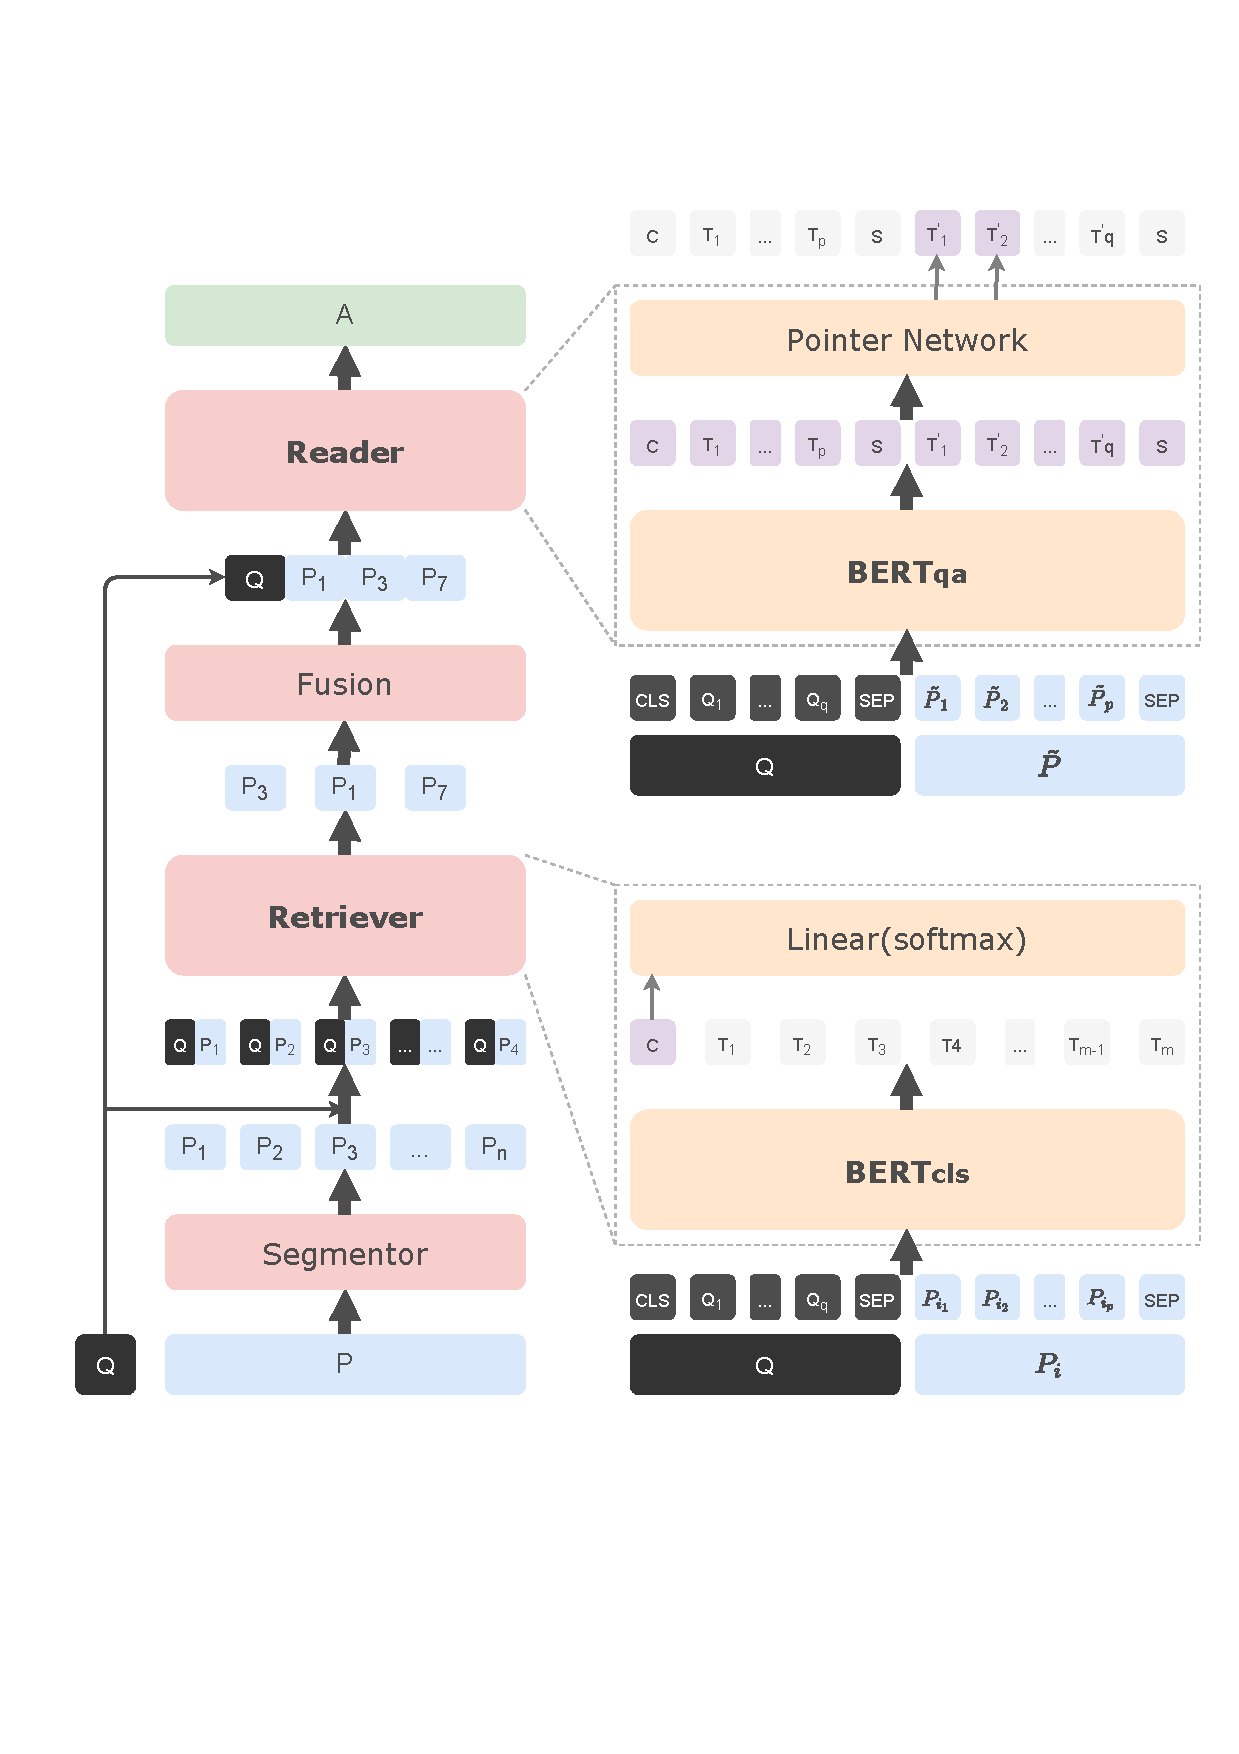
\includegraphics [width=0.8\textwidth] {figure/3-1.pdf}
        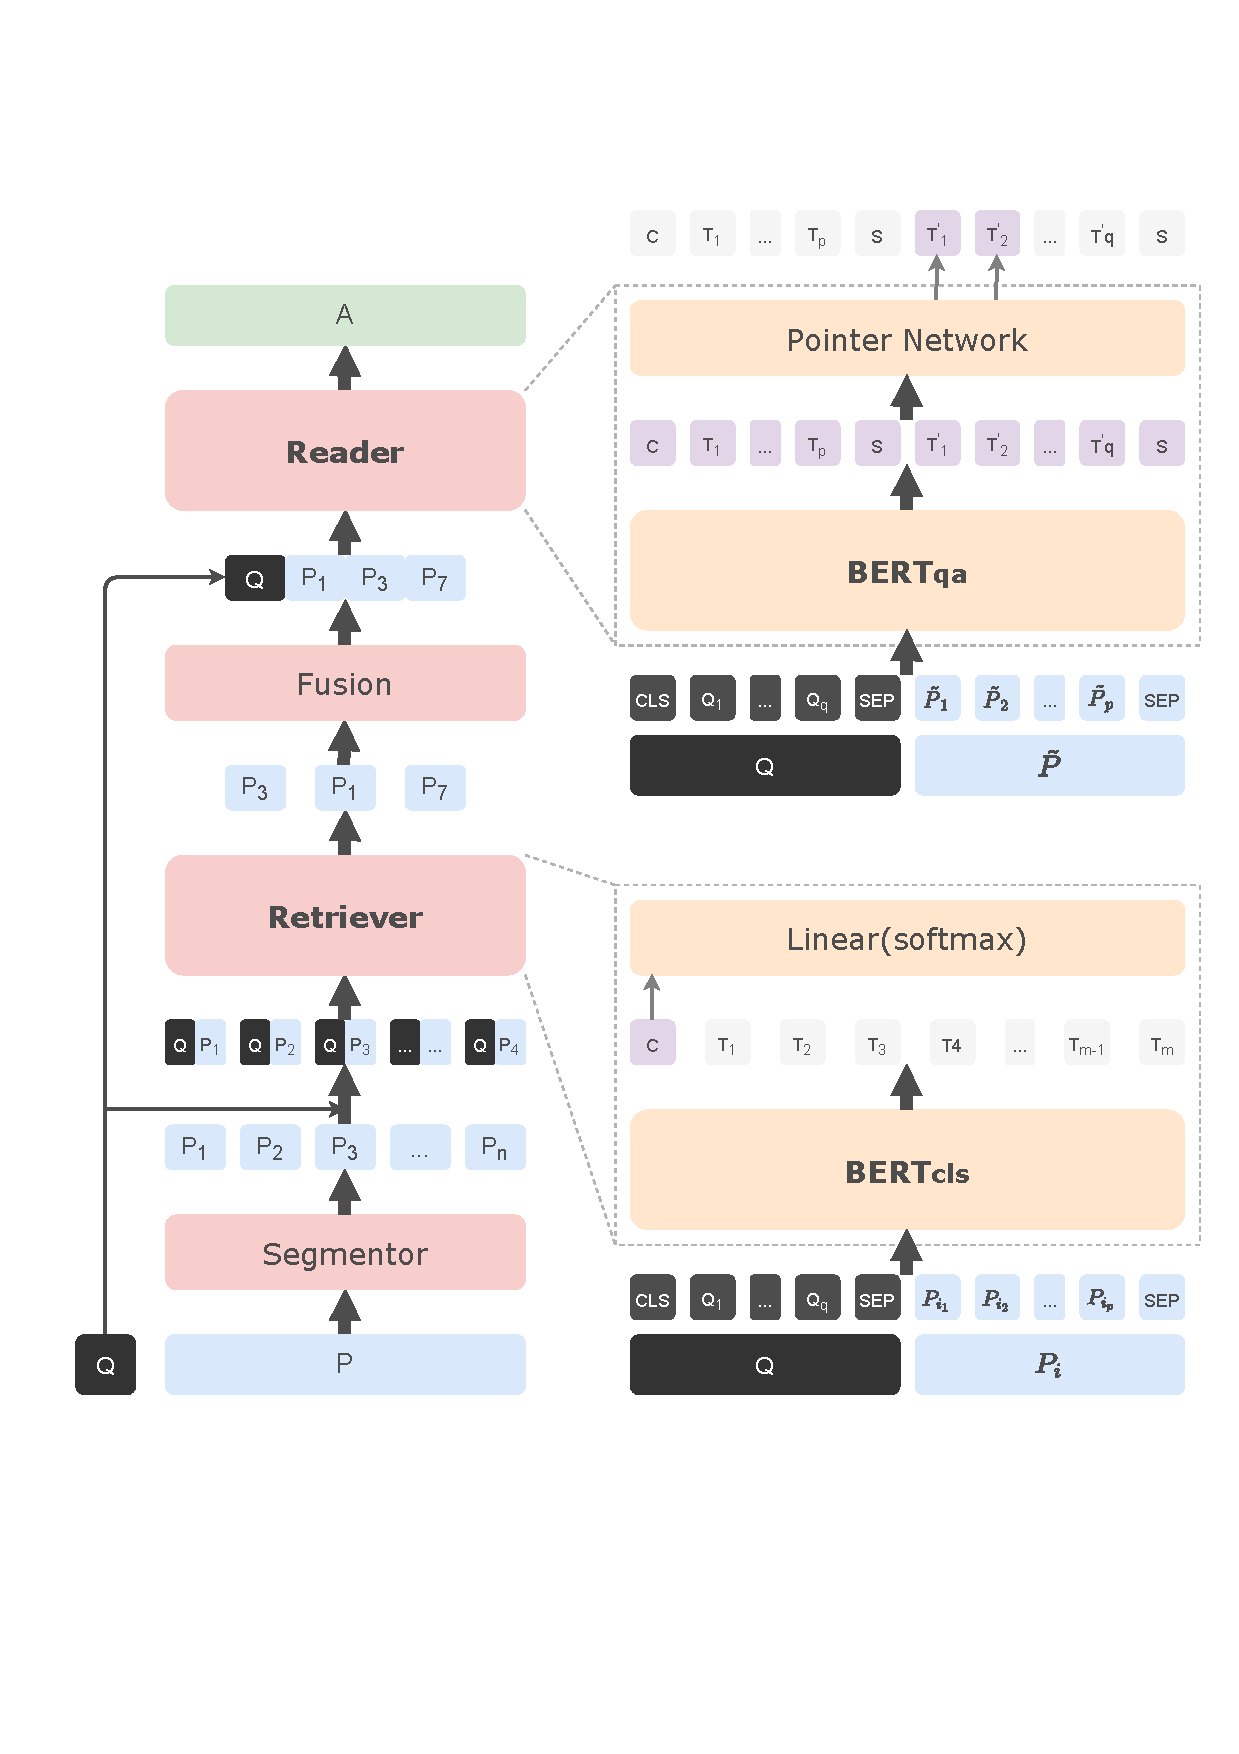
\includegraphics[scale=0.6]{figure/3-1.pdf}
    \caption{ThinkTwice的基本架构}
    \label{fig:3-1}
\end{figure}


\subsection{分段方法}
长文本阅读理解的主要挑战在于如何在给定文章中的大量知识片段中准确地定位到最重要的信息。
这些文章的长度通常超过现有神经网络模型所能容纳的最大长度(例如512个token)。
为了应对这个问题,我们在NewsQA数据集中为每篇文章的结尾添加了一个分割标记。
通过这种方式,可以将输入文本$P$分割成文本片段$P_1,P_2,...,P_n$,其中每个文本片段的长度限制在60-80个token左右。
这种形式化的分割方法可以有效地提高模型的处理效率和准确性。

\subsection{基于预训练语言模型的段落检索器}
当人们需要从大量文本中寻找答案时,通常会选择保留与当前问题最相关的文本片段,并过滤掉琐碎的信息。
受到这种人类行为的启发,本文提出了一个基于预训练语言模型的检索器,来选择最有可能回答问题的最重要的文本片段。

具体而言,检索器部分首先将问题$Q$和每个文本片段$\{P_i\}^n_{i=1}$组合成多个序列$\{x_i\}^n_{i=1}$,其中$x_i=[CLS]Q[SEP]P_i[SEP]$\footnote{[CLS]和[SPE]是特殊token。前者对于编码后的输入序列,理论上可以表示整体信息;后者主要用于分隔输入序列}。
然后,检索器的编码器部分,也就是预训练语言模型,用于将输入$x_i$编码成整个序列的上下文词嵌入表示$H_i$:
\begin{equation}
    H_i = BERT_{cls}(x_i).
\end{equation}

[CLS]的隐向量表示$H^{cls}_i$代表了整个序列的总体表示。
然后,一层线性网络和Softmax层用于得到该序列的分类概率$\hat y_c$:
\begin{equation}
    \hat y_c=Softmax(Linear(H_i^{cls})),
\end{equation}

其中$\hat y_c$表示当前文本片段$P_i$是否包含可以回答给定问题的有效信息\cite{zhang2020retrospective}。
在训练阶段,当$P_i$包含标注答案时,“有/无答案”标签$y_{c(i)}$设为1,否则设为0。

交叉熵损失函数用于计算真实答案$y_c$和预测概率$\hat y_c$之间的损失:
\begin{equation}
    \mathcal  L_{retriever}  = -\frac{1}{n}\sum_{i=1}^{n}[y_{c(i)}\log\hat y_{c(i)}+(1-y_{c(i)})log(1-\hat y_{c(i)})].
\end{equation}

\subsection{融合方法}
上一小节利用检索器得到了输出概率值$\{\hat y_{c(i)}\}^n_{i=1}$,该值可以量化每个文本片段$\{P_i\}^n_{i=1}$回答给定问题$Q$的可能性大小。
接下来,根据$\hat y$的值,选择与问题$Q$最相关的$k$个文本片段,并舍弃其他片段。
被选中的文本片段按照它们在原文中的顺序合并成单个序列,以确保整个组合文本的语义连贯性和上下文连续性。
例如,当$k=3$且分数最高的3个文本片段分别是$P_3$,$P_1$和$P_7$时,融合器需要根据它们在原文中的相对顺序将它们拼接在一起。
对于可能出现的特别长的文本,融合器可以直接对其进行截断。
因此,融合器的输出可以表示为图~\ref{fig:3-1}~中的$\tilde P=<P_1,P_3,P_7>$。

\subsection{基于与预训练语言模型的阅读理解模型}
通过以上模块,已经从原始的长文本$P$中提取了一段短文本$\tilde P$。
本节中的阅读器模块首先将问题$Q$和上一节得到的$\tilde P$拼接成一个单独的序列$z=[CLS]Q[SEP]\tilde P[SEP]$,随后使用另一个预训练语言模型BERT\cite{devlin2018bert}作为阅读器的编码器,将输入$z$映射到一个上下文隐向量序列。
下一步,指针网略将问题相关的文本表示的答案片段的起始和结束位置进行解码:
\begin{equation}
    \mathcal L_{reader} = \frac{1}{2} CrossEntropy(\hat y_s,y_s) + \frac{1}{2} CrossEntropy(\hat y_e,y_e)
\end{equation}

其中$\hat y_s$和$\hat y_e$分别表示由阅读器解码的预测答案的起始和结束位置的概率。

在训练过程中,阅读器中使用了交叉熵损失来计算起始和结束位置的损失:
\begin{equation}
    \mathcal L_{reader} = \frac{1}{2} CrossEntropy(\hat y_s,y_s) + \frac{1}{2} CrossEntropy(\hat y_e,y_e)
\end{equation}
其中,$y_s$和$y_e$分别表示开始和结束位置的标签。
如果当前段落给出的信息不能回答问题,$y_s$和$y_e$都设为0,也就是指向$[LCS]$token。
在预测阶段,阅读器首先计算“有答案”分数$score_{has}$和“无答案”分数$score_{null}$,各自用$\hat y_s$和$\hat y_e$来表示:
\begin{equation}
    score_{has}=\max \limits_{1\le i\le j<L}(\hat y_{s}^{(i)}+\hat y_{e}^{(j)})
\end{equation}
\begin{equation}
    score_{null}=\hat y_{s}^{(0)}+\hat y_{e}^{(0)}
\end{equation}
其中$i$和$j$表示在整个序列长度$L$内的答案位置,并且由于起始位置一定在结束位置之前,有$i$一定限制为小于$j$。
另外,鉴于序列首部的$[CLS]$不表示$\tilde P$中的任何词,$\hat y^{(0)}_s$和$\hat y^{(0)}_e$表示整个文本没有答案的概率。

接下来,通过计算$score_{has}$和$score_{null}$之间的距离来计算两者之间的距离分数$score_{dist}$,以此作为“有/无答案”的依据:
\begin{equation}
    score_{dist}=score_{null}-score_{has}
\end{equation}
\begin{equation}
    s,e=\argmax \limits_{1\le i\le j<L}(\hat y_{s}^{(i)}+\hat y_{e}^{(j)})
\end{equation}
其中有一个阈值$\delta$,如果$score_{dist}$小于$\delta$,阅读器输出的$s$和$e$就代表了答案的起始和结束位置,否则阅读器会将该问题视为一个不可回答问题。

\section{实验及结果分析}

\subsection{实验设置}
本章在一个具有挑战性的长篇文本阅读理解数据集NewsQA上进行了实验。
该数据集包含来自CNN的13,000篇新闻文章,以及120,000条人工生成的问题答案对。
在排除了20,000条标注者认为没有意义的低质量问题后,本章对剩余的数据进行了实验分析。
因此,NewsQA的训练/开发/测试集分别包含90,000/5,000/5,000条问题答案对。
此外,本章还具体统计了每篇文章的token数量(即tokens per passage, TPP)和每篇文章的段落数量(即paragraphs per passage, PPP)。
在训练/开发/测试集上,TPP的中位数分别为774/734/707,最大值分别为3,100/2,300/2,300。
而PPP在三个集上的中位数为18/18/17,最大值为87/63/54。

针对NewsQA数据集,存在一些长文本模型。
\begin{itemize}
    \item Match-LSTM\cite{wang2015learning}。该模型使用了两个单向的LSTM来编码问题和文章。
    \item BiDAF\cite{seo2016bidirectional}。BIDAF的核心思想是其中的双流注意力层,双流注意力分别计算上下文之于问题的注意力以及问题之于上下文的注意力。
    \item AMANDA\cite{kundu2018question}。AMANDA针对答案抽取提出了一种端到端的专注于问题的多因子注意力网络。多因子注意力编码聚合了位于多个句子中有意义的事实。
    \item DecaProp\cite{tay2018densely}。该模型把自注意力网络整合进RNN模\cite{mikolov2010recurrent}型。
    \item Longformer\cite{beltagy2020longformer}。该预训练语言模型使用了稀疏注意力矩阵,来解决序列长度的限制。
    \item CogLTX\cite{ding2020cogltx}。CogLTX架构通过判别多个句子间的相关性来识别重要句子。
\end{itemize}

本章采用EM和F1这两个官方指标来衡量长文本机器阅读理解的性能。
其中,EM指标用于衡量预测答案与真实答案完全匹配的比例,而F1指标则用于衡量预测答案与真实答案在token级的平均重叠程度。

为了验证两阶段阅读策略的有效性,本章使用了部分预训练语言模型,并采用将文章划分成多个段落的滑动窗口机制来处理长文本阅读理解问题。
所采用的预训练语言模型包括BERT\cite{devlin2018bert}、RoBERTa\cite{liu2019roberta}、ALBERT\cite{lan2019albert}和SpanBERT\cite{joshi2020spanbert},这些模型均基于Transformer\cite{vaswani2017attention}架构,且使用PyTorch实现。
在训练阶段,基础模型的学习率设为2e-5,而大模型的学习率则设为2e-6。此外,热身比例设为0.1,L2权重衰减设为0.01。
批量尺寸在基础模型中为8,在大模型中为1。
对于检索器,轮次数量在基础模型中设为1,在大模型中设为2;
而阅读器中这个值保持为3。
在分词方面,本章采用wordpieces\cite{wu2016google}进行分词,并将第一阶段的最大长度设为256,第二阶段的最大长度设为512。
第一阶段中进行了大量实验,用来选择$k$值\footnote{$k$值是一个超参数,表示检索器筛选出的最好的$k$个段落。}。

\begin{table}[]
    \centering
    \caption{The performances of LT-MRC models on NewsQA as well as our models' performances compared to their corresponding pre-trained language models.}
    \begin{tabular}{p{140pt}p{24pt}<{\centering}p{24pt}<{\centering}p{24pt}<{\centering}p{24pt}<{\centering}}
        %  \thickhline
         \hline
         {\bfseries Model} & \multicolumn{2}{c}{\bfseries Dev} & \multicolumn{2}{c}{\bfseries Test} \\
         & {\bfseries F1} & {\bfseries EM} & {\bfseries F1} & {\bfseries EM} \\
         \hline
         Match-LSTM~\cite{wang2015learning} & 49.6 & 34.4 & 50.0 & 34.9 \\
         BiDAF~\cite{seo2016bidirectional} & - & - & 52.3 & 37.1 \\
         AMANDA~\cite{kundu2018question} & 63.3 & 48.8 & 63.7 & 48.4 \\
         DecaProp~\cite{tay2018densely} & 65.7 & 52.5 & 66.3 & 53.1 \\
         Longformer-base~\cite{beltagy2020longformer} & 68.1 & 58.3 & 68.1 & 58.1 \\
         CogLTX~\cite{ding2020cogltx} & - & - & 70.1 & 55.2 \\
         \hline
         \hline
         BERT-base~\cite{devlin2018bert} & 65.6 & 56.3 & 65.4 & 55.2 \\
         $\ $ + ThinkTwice(descending order) & 66.6 & 57.8 & 65.8 & 55.6 \\
         $\ $ + ThinkTwice(ours) & {\bfseries 68.5} & {\bfseries58.8} & {\bfseries68.6} & {\bfseries57.7} \\
         \hline
         RoBERTa-base~\cite{liu2019roberta} & 63.7 & 53.5 & 63.2 & 53.1 \\
         $\ $ + ThinkTwice(ours) & {\bfseries67.7} & {\bfseries58.6} & {\bfseries67.7} & {\bfseries58.4} \\
         \hline
         ALBERT-base~\cite{lan2019albert} & 68.1 & 58.2 & 68.0 & 58.0 \\
         $\ $ + ThinkTwice(ours) & {\bfseries68.7} & {\bfseries59.1} & {\bfseries68.6} & {\bfseries58.8} \\
         \hline
         SpanBERT-base~\cite{joshi2020spanbert} & 67.7 & 57.1 & 67.5 & 56.2 \\
         $\ $ + ThinkTwice(ours) & {\bfseries69.9} & {\bfseries59.8} & {\bfseries69.7} & {\bfseries59.4} \\
         \hline
         BERT-large & 68.9 & 59.2 & 68.8 & 58.6 \\
         $\ $ + ThinkTwice(ours) & {\bfseries70.1} & {\bfseries59.5} & {\bfseries69.8} & {\bfseries59.4} \\
         \hline
         SpanBERT-large & 71.2 & 61.8 & 70.9 & 59.8 \\
         $\ $ + ThinkTwice(ours) & {\bfseries72.1} & {\bfseries62.2} & {\bfseries71.5} & {\bfseries61.0} \\
        %  \thickhline
         \hline
    \end{tabular}
    \label{tab:3-1}
\end{table}


\subsection{实验结果和分析}
\textbf{与现有模型相比}。
表~\ref{tab:3-1}~呈现了ThinkTwice模型与现有模型的比较结果。
该表说明,本章提出的模型在NewsQA数据集上表现卓越,超越了现有的长文本阅读理解模型。
具体而言,在EM指标上,本模型相比现有模型提升了5.8个百分点,在F1指标上提升了1.4个百分点。
此外,实验结果也同样表明,实现ThinkTwice策略可以提高所有预训练阅读理解模型的性能。
例如,在BERT-base模型上,F1值提高了3.2个百分点,在RoBERTa-base模型上,F1值提高了4.5个百分点。
然而,在ALBERT-base模型上的提升并不显著。
这可能有两个原因:首先,ALBERT模型中的句子顺序预测(sentence-order prediction,SOP)预训练任务已经解决了句子内部连贯性的问题;
其次,ALBERT模型中实现了跨层参数共享机制,导致即使实现了新的策略,参数变化也非常微小。
在其他模型上实验性能的大幅提升表明,ThinkTwice策略中的检索器精准地抽取了最重要的段落,从而将长文本压缩成合适长度的短文本,同时最大程度地保留了原始文本中最重要的信息。

此外,为了研究不同融合方式对最终性能的影响,本章还尝试在BERT-base模型上采用两种不同的融合策略来合并筛选出的文本片段。
其中一种方法是将检索器提取出的文本片段按照与给定问题的相关性进行降序排列并进行合并;
另一种方法是按照先前所述的方法,以原文的顺序进行合并。
从表格~\ref{tab:3-1}~中的第8行和第9行可以发现,原始的融合方式要显著优于降序的融合方式(提升2.8),尽管采用降序方式排列的模型也超出了基线模型(0.4)。
这个对比实验表明,扰乱序列顺序可能会导致上下文信息的丢失。

\begin{figure}[htbp]
    \centering
    % 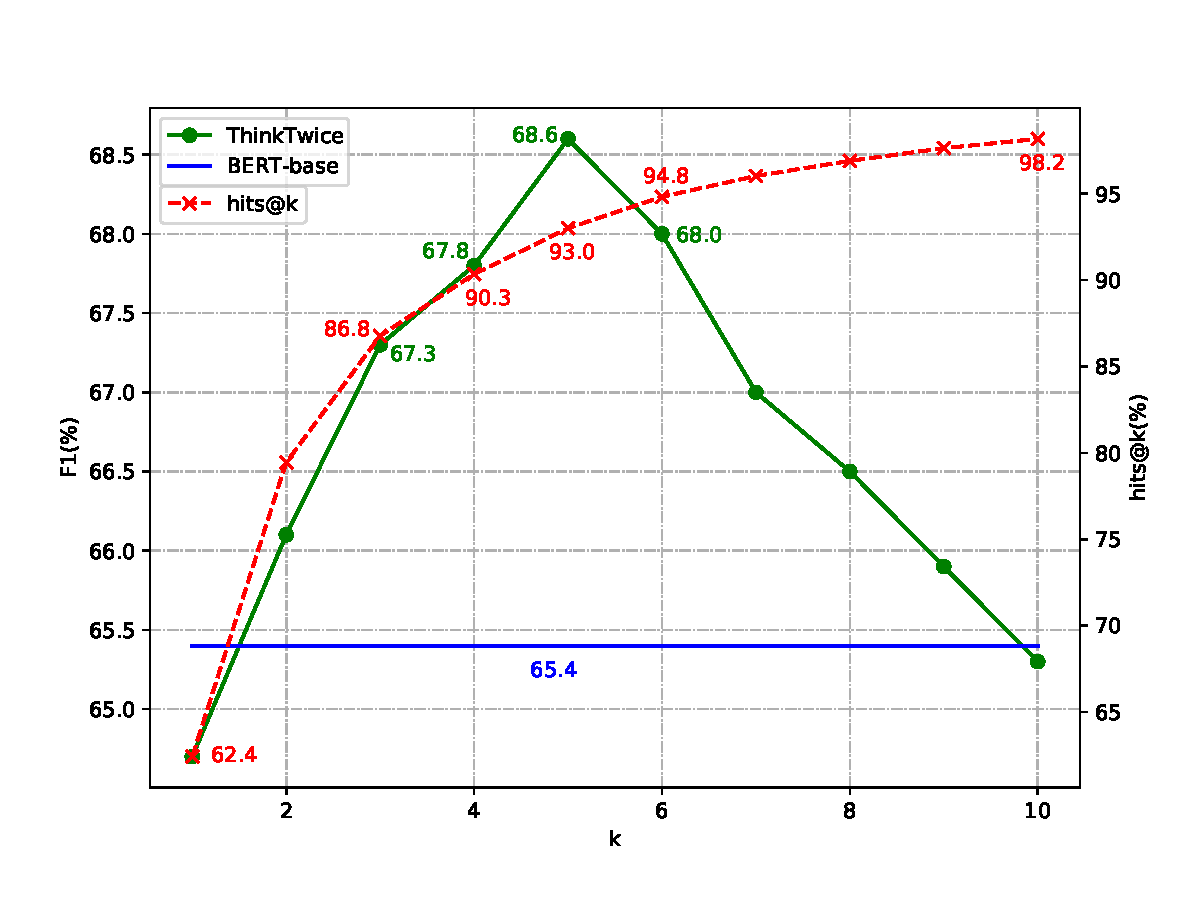
\includegraphics[width=\textwidth]{figure/3-2.pdf}
    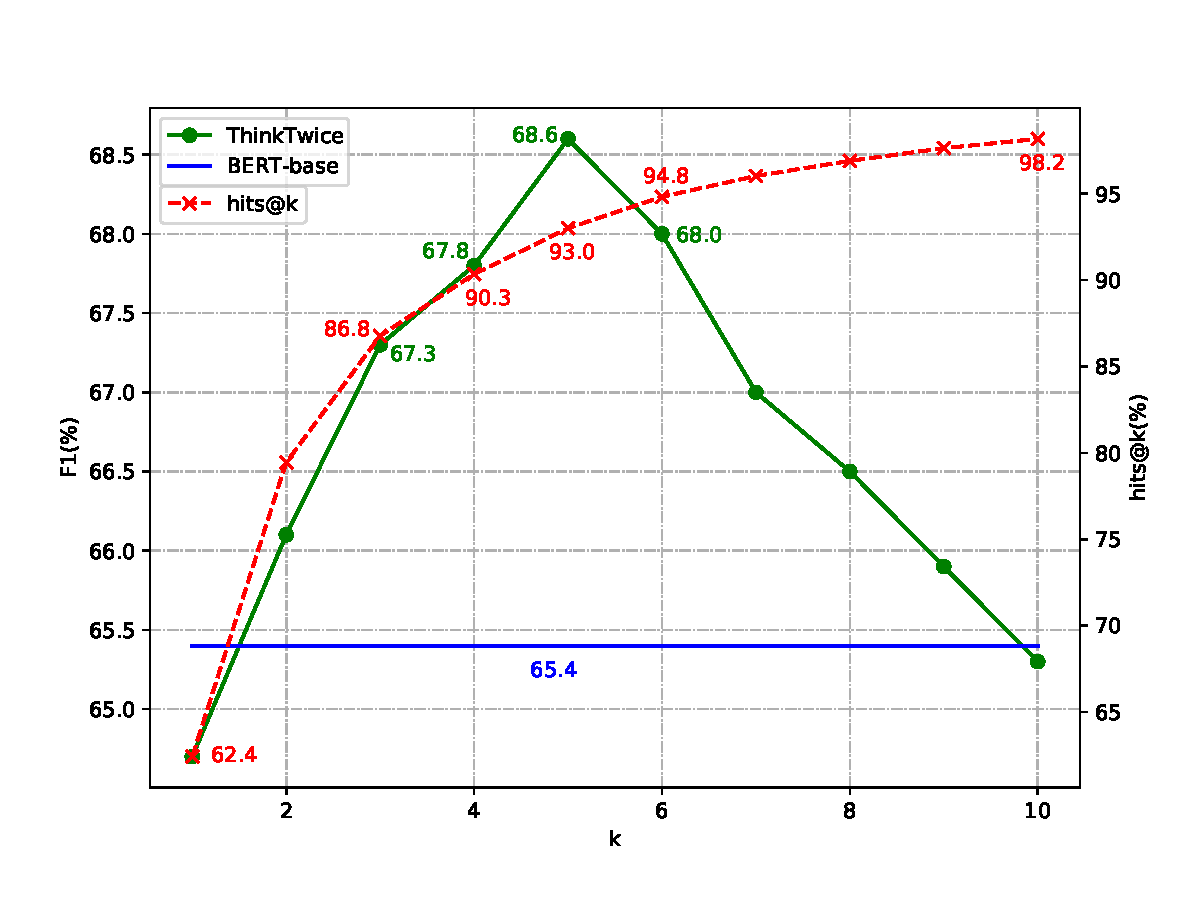
\includegraphics[scale=0.7]{figure/3-2.pdf}
    \caption{在不同$k$值情况下,检索器和ThinkTwice模型(基于BERT-base)的性能关联}
    \label{fig:3-2}
\end{figure}

\begin{figure}
    \centering
    % 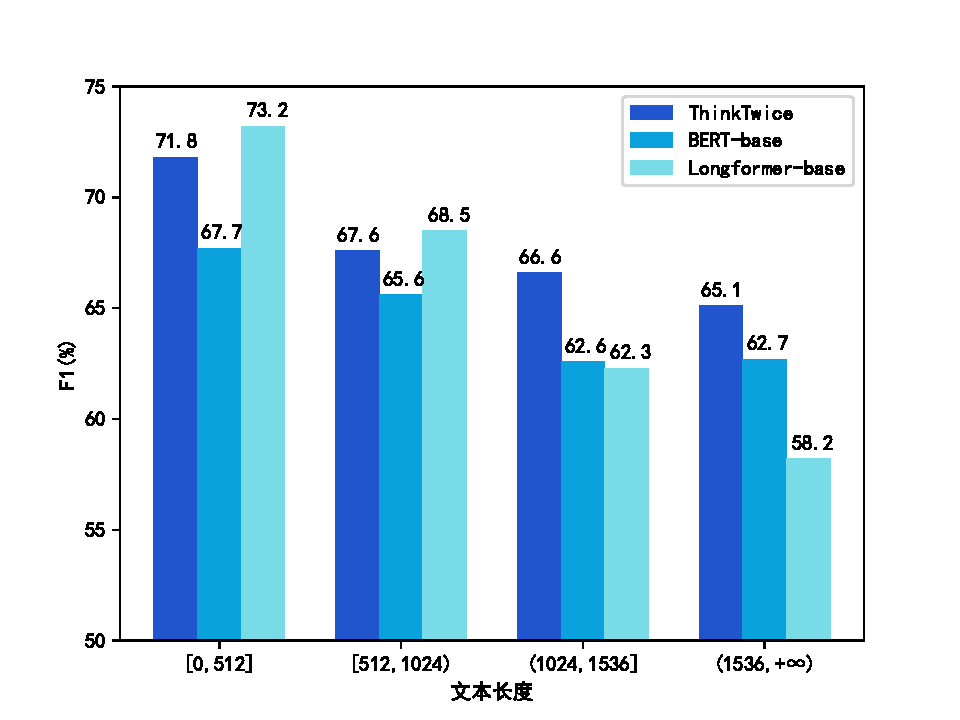
\includegraphics[width=0.7\textwidth]{figure/3-3.pdf}
    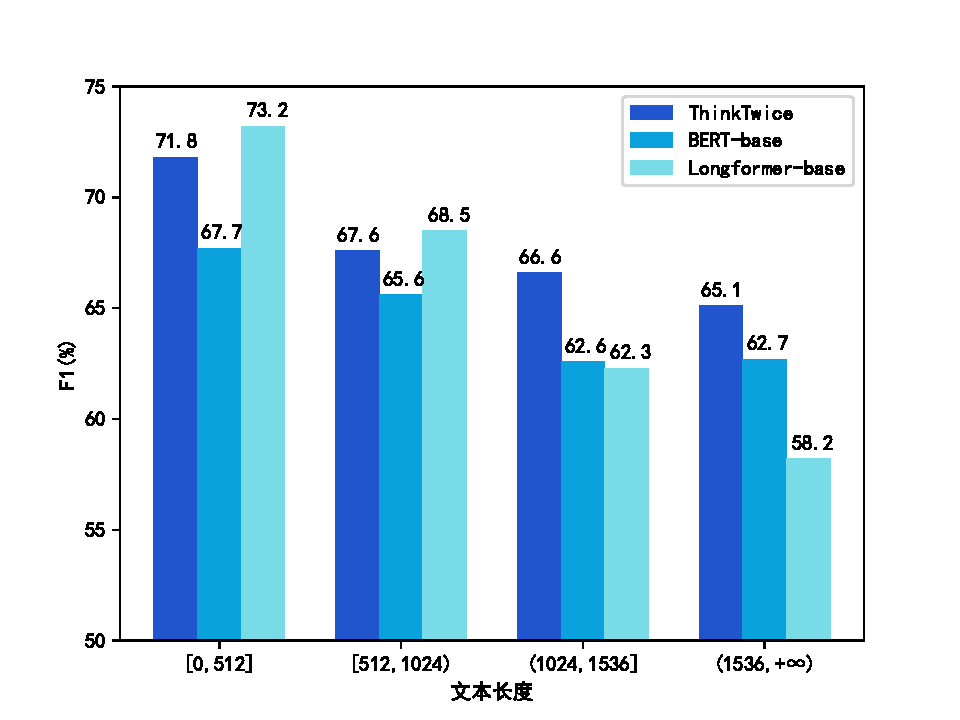
\includegraphics[scale=0.7]{figure/3-3.pdf}
    \caption{Performances of ThinkTwice, BERT-base, and Longformer-base over different text lengths. The number of samples in the four length intervals are: 1,611, 2,074, 1,089, and 210.}
    \label{fig:3-3}
\end{figure}


\textbf{段落检索}。
图~\ref{fig:3-2}~展示了检索器的不同参数配置与ThinkTwice模型之间的关系。
对于检索器,评估指标Hits@$k$(前$k$个最准确的)衡量了检索器筛选出的最佳$k$个段落是否包含真实答案。
对于ThinkTwice模型,F1评估NewsQA数据集上阅读理解模型的最终性能。
红色曲线表明,$k$值越大,Hits@$k$准确率就越高。同时,当$k$大于3时,检索器的该项指标也超过了90\%。
此外,当$k$等于5时,ThinkTwice模型(绿色曲线)实现了最佳性能(68.6)。
这表明,当$k$值较小时,检索器无法召回足够多的备选段落;
当$k$大于5时,更多的备选段落需要搜索更大的文本范围,从而导致性能下降。
因此,ThinkTwice在所有实验中将超参数$k$设为5。
本节还将ThinkTwice模型与相应的BERT-base阅读理解模型(蓝色曲线)进行了比较。
结果显示,当$k$设为2到9之间时,ThinkTwice模型的表现优于BERT-base,这验证了ThinkTwice两阶段策略的有效性。

\textbf{文本长度的作用}。
为了验证ThinkTwice在长文本领域的作用,本节将对多个不同长度的文本进行测试,并将测试结果与BERT-base和Longformer-base等阅读理解模型进行比较。
值得注意的是,这里ThinkTwice模型的阅读器应用了BERT-base。
图~\ref{fig:3-3}~列出了实验结果。
可以看到,在较短的文本长度范围内([0,512]和(512,1024]),Longformer实现了最好的实验结果。
其中的原因是Longformer-base继承了RoBERTa的预训练参数权重,而这些参数已经在阅读理解任务中表现得很好。
然而,在较长的文档长度范围内((1024,1536],(1536,$+\infty$)),本章提出的ThinkTwice模型显著优于其他模型。
这也证实了ThinkTwice能够准确地定位到包含答案的文本片段。
此外,在较长文档的实验结果中,BERT-base也要优于Longformer-base,这表明滑动窗口机制(BERT-base)相较于直接的长文本输入(Longformer-base),也有一定优势。
最后可以发现,随着文档长度的增加,ThinkTwice模型的性能是最稳定的,特别是当文本长度大于512的时候。

\begin{table}[htbp]\scriptsize
    \centering
    \caption{NewsQA数据集上两个关于三个基线模型和CoLISA模型的预测的例子}
    \begin{tabular}{p{408pt}}
        \hline
        \multicolumn{1}{c}{\bfseries 例子1} \\
        \hline
        文章:\\
        (CNN) -- President Barack Obama spoke with Egypt's president moments after Hosni Mubarak addressed his country, telling the Egyptian that \textcolor[rgb]{1,0,0.2}{he must make good on his promises} and avoid a violent response to the thousands of protesters in the streets. (...) \\
        <译文:(...) 巴拉克·奥巴马总统在穆巴拉克发表讲话后不久与埃及总统进行了交谈,告诉埃及总统他必须履行承诺,避免对街头上万名抗议者采取暴力行动。(...) > \\
        \hline
        Token数量:2,036 \\
        \hline
        问题:\\
        What did Obama say to Mubarak? \\
        <译文:奥巴马对穆巴拉克说了什么?> \\
        \hline
        答案:\\
        he must make good on his promises \\
        <译文:他必须遵守诺言> \\
        \hline
        CoLISA预测:\\
        \textcolor[rgb]{1,0,0.2}{he must make good on his promises and avoid a violent response} (True) \\
        <译文:他必须遵守诺言并避免采取暴力行动> \\
        \hline
        BERT预测:\\
        I just spoke to him after his speech (False)
        <译文:我在他演讲结束以后跟他讲过> \\
        \hline
        ALBERT预测:\\
        It is very important that people have mechanisms in order (False) \\
        <译文:人们拥有机制非常重要> \\
        \hline
        Longformer预测:\\
        he must make good on his promises and avoid a violent response (True) \\
        <译文:他必须遵守诺言并避免采取暴力行动> \\
        \hline
        % \hline
        \multicolumn{1}{c}{\bfseries 例子2} \\
        \hline
        文章:\\
        (...) Tucked away in the verdant hills west of St. Andrews, Kingarrock Hickory Golf Course (greens fee, \$40 for nine holes and \$55 for 18) \textcolor[rgb]{1,0,0.2}{is a nine-hole, 2,022-yard country estate course that is played exclusively with antiquated equipment}. (...) \\
        <译文:(...) 坐落在圣安德鲁斯西部郁郁葱葱的山丘上,Kingarrock Hickory高尔夫球场(九洞的场地费为40美元,18洞的场地费为55美元)是一个九洞、2022码的乡村庄园球场,球场上全部使用古董设备打球。(...) > \\
        \hline
        Token数量:2,288 \\
        \hline
        问题:\\
        What is Kingarrock Hickory? \\
        <译文:Kingarrock Hickory是什么?> \\
        \hline
        答案:\\
        is a nine-hole, 2,022-yard country estate course that is played exclusively with antiquated equipment \\
        <译文:是一个九洞、2022码的乡村庄园球场,球场上全部使用古董设备打球> \\
        \hline
        CoLISA预测:\\
        \textcolor[rgb]{1,0,0.2}{a nine-hole, 2,022-yard country estate course that is played exclusively with antiquated equipment} (True) \\
        % CoLISA预测:\underline{a nine-hole, 2,022-yard country estate course that is played exclusively with antiquated equipment (True)} \\
        <译文:一个九洞、2022码的乡村庄园球场,球场上全部使用古董设备打球> \\
        \hline
        %  BERT预测:\textcolor[rgb]{0.4,0.7,0.9}{the kind of place that can change the way one thinks about golf (False)} \\
        BERT预测:\\
        the kind of place that can change the way one thinks about golf (False) \\
        <译文:一种可以改变人们对高尔夫球看法的地方> \\
        \hline
        ALBERT预测:\\
        Golf Course (True)
        <译文:高尔夫球场> \\
        \hline
        Longformer预测: \\
        Top hotel penthouses (False)
        <译文:顶级酒店顶层套房> \\
        \hline
    \end{tabular}
    \label{tab:3-2}
\end{table}


本章节还进行了一个案例分析,以进一步比较NewsQA上ThinkTwice模型的预测结果与其他模型之间的差异。
研究结果表明,ThinkTwice模型的预测答案与真实答案更加接近。

为了验证模型在处理特别长的文本上的性能,本章节选取了两篇长度超过2,000词的文章作为样例,如表~\ref{tab:3-2}~所示。
在例子1中,模型需要回答奥巴马说了什么,ThinkTwice准确地定位到包含最终答案的第一段段落,并给出了奥巴马说出的合适内容。
然而,BERT和ALBERT却没有像预期那样表现出色,它们分别抽取了其他段落的句子。
在例子2中,ThinkTwice模型同样准确地定位到了正确的段落,而BERT和Longformer的表现则不尽如人意。


\section{本章小结}
本章提出了一种二阶段方法,用于在长文本阅读理解任务中解决预训练语言模型中的长度限制问题。
ThinkTwice模型通过将长文本压缩为较短的文本形式,并准确定位答案位置来实现这一目标。
实验结果和分析表明,该方法在长文本任务上具有有效性。
然而,该方法存在一个潜在的缺陷,即由检索器压缩得到的短文本可能因缺乏先行词而导致不连贯。
因此,未来的研究将集中于通过指代消解或位置词嵌入等方式来解决这个问题。


